% FEB Composites app: quick start guide.
% Build with:  lualatex quick-start.tex   (needs the img/ folder beside it)
% Screenshots are of the real app (v6.1.0) running on the test fixtures, so
% every name and number in them is sample data.
\documentclass[11pt]{article}
\usepackage[letterpaper,margin=0.8in,top=0.7in,bottom=0.8in]{geometry}
\usepackage{fontspec}
\setmainfont{Helvetica Neue}[BoldFont={Helvetica Neue Bold}]
\newfontfamily\headfont{Avenir Next}[Ligatures=TeX,UprightFont={* Demi Bold},BoldFont={* Heavy}]
\usepackage{xcolor}
\usepackage{graphicx}
\usepackage[most]{tcolorbox}
\usepackage{tikz}
\usepackage{enumitem}
\usepackage{array}
\usepackage{fancyhdr}
\usepackage[hidelinks]{hyperref}
\graphicspath{{img/}}

\definecolor{navy}{HTML}{0F2D52}
\definecolor{feblue}{HTML}{2F6BE4}
\definecolor{gold}{HTML}{FDB515}
\definecolor{paleblue}{HTML}{E9EEF5}
\definecolor{tipblue}{HTML}{DCE8F8}
\definecolor{ink}{HTML}{1F2937}
\definecolor{muted}{HTML}{5B6573}
\color{ink}

\setlength{\parindent}{0pt}
\setlength{\parskip}{6pt}
\linespread{1.12}

\pagestyle{fancy}
\fancyhf{}
\renewcommand{\headrulewidth}{0pt}
\fancyfoot[L]{\small\color{muted}FEB Composites app $\cdot$ quick start}
\fancyfoot[R]{\small\color{muted}\thepage}

% glyph inline: \g{name}
\newcommand{\g}[1]{\raisebox{-0.22em}{\includegraphics[height=1.15em]{ic-#1}}}
\newcommand{\key}[1]{\tikz[baseline=(k.base)]\node[draw=muted!60,fill=paleblue,rounded corners=2pt,inner sep=2pt,font=\small](k){#1};}

% numbered section badge, like the app's own mockup frames
\newcommand{\step}[2]{%
  \vspace{4pt}%
  {\headfont\Large
   \tikz[baseline=(b.base)]\node[circle,fill=navy,text=white,minimum size=1.5em,inner sep=0pt,font=\headfont\large](b){#1};%
   \hspace{0.35em}\textcolor{navy}{#2}}\par\vspace{2pt}}

\newtcolorbox{tip}[1][Tip]{colback=tipblue,colframe=tipblue,coltext=navy,
  arc=6pt,boxrule=0pt,left=10pt,right=10pt,top=6pt,bottom=6pt,
  fontupper=\small\raggedright,before upper={\textbf{#1.}\ }}

\newtcolorbox{shot}{colback=white,colframe=navy!15,arc=8pt,boxrule=0.6pt,
  left=0pt,right=0pt,top=0pt,bottom=0pt,
  enhanced,drop shadow={navy!25}}

\begin{document}

%% ---------------------------------------------------------------- cover strip
\begin{tcolorbox}[colback=navy,colframe=navy,arc=10pt,left=16pt,right=16pt,top=14pt,bottom=14pt]
\begin{minipage}{0.12\linewidth}
  
\includegraphics[width=\linewidth]{febmark}
\end{minipage}\hfill
\begin{minipage}{0.84\linewidth}
  {\headfont\color{white}\fontsize{26}{30}\selectfont FEB \textcolor{gold}{Composites}}\\[3pt]
  {\color{white}\large Quick start. Five minutes, and you're in.}
\end{minipage}
\end{tcolorbox}

\vspace{4pt}
The composites app is where the team keeps track of everything we build: parts,
molds, the runs that make them, what's on the shelf, and who signed what. You
don't need to learn all of it. Most people use three things: the
\textbf{Dashboard}, a \textbf{Work Order}, and the \textbf{buy-off button}.
This sheet covers those.

\begin{tip}[Relax]
You can't break anything by looking around. Clicking a tab, opening a record,
or scrolling changes nothing. Edits only happen when you press \textbf{Edit} or
a buy-off button, and a lead can fix anything that goes wrong.
\end{tip}

%% ---------------------------------------------------------------- 1 get in
\step{1}{Get in}

\begin{minipage}[t]{0.52\linewidth}
\vspace{0pt}
\begin{enumerate}[leftmargin=1.4em,itemsep=4pt]
  \item Open \href{https://feb-composites.web.app}{\textcolor{feblue}{\textbf{feb-composites.web.app}}}
        on your laptop or phone.
  \item Press \textbf{New here? Create account}.
  \item Type your real name (it goes on everything you sign), pick a username
        and a password.
  \item That's it. You're a member and can start working straight away.
\end{enumerate}

Just curious? \textbf{View as guest} shows the whole app read-only, no account
needed.

\begin{tip}[On your phone]
In the browser's share menu, choose \emph{Add to Home Screen}. The app then
opens like any other app, which is handy at RFS.
\end{tip}
\end{minipage}\hfill
\begin{minipage}[t]{0.42\linewidth}
\vspace{0pt}
\begin{shot}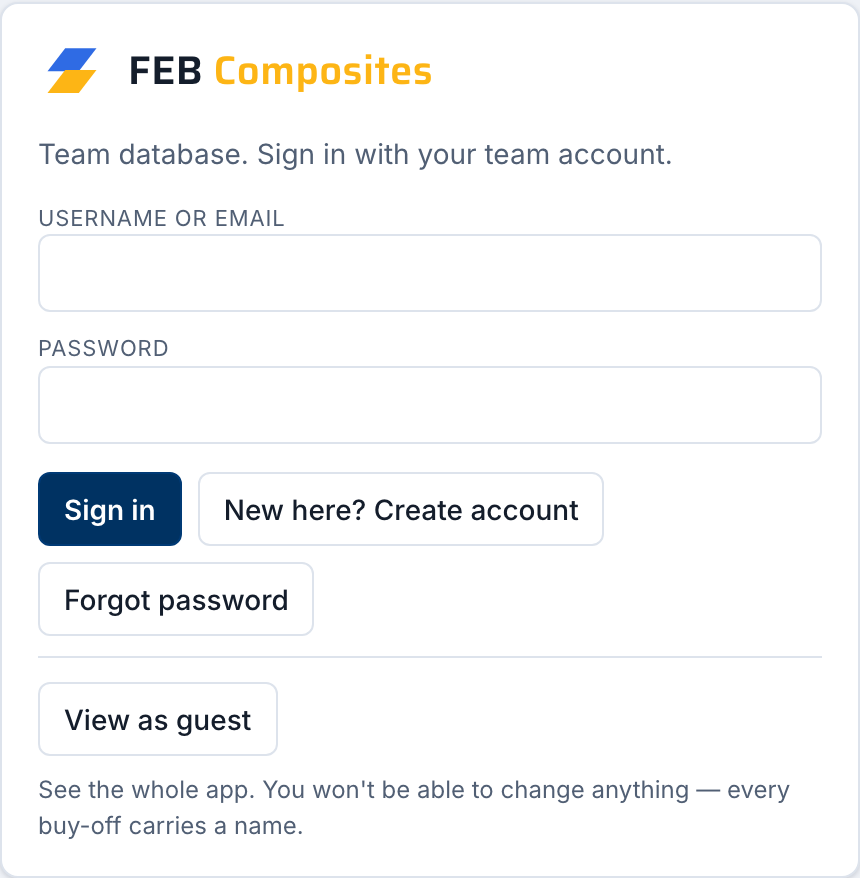
\includegraphics[width=\linewidth]{login}\end{shot}
\end{minipage}

\newpage
%% ---------------------------------------------------------------- 2 around
\step{2}{Find your way around}

The blue sidebar on the left is every section of the app. You'll live in the
first few; the rest are there when you need them.

\begin{minipage}[t]{0.25\linewidth}
\vspace{0pt}
\begin{shot}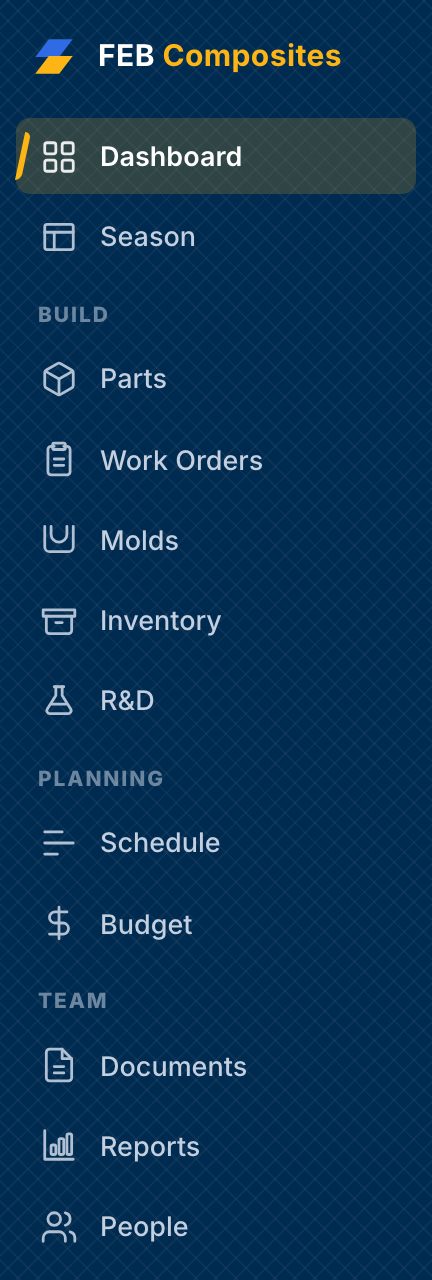
\includegraphics[width=\linewidth]{sidebar}\end{shot}
\end{minipage}\hfill
\begin{minipage}[t]{0.71\linewidth}
\vspace{0pt}
\renewcommand{\arraystretch}{1.45}
\begin{tabular}{@{}c@{\hspace{8pt}}>{\bfseries}l@{\hspace{10pt}}>{\raggedright\arraybackslash}p{0.6\linewidth}@{}}
\g{dashboard} & Dashboard   & What needs doing, today. \textbf{Start here.}\\
\g{season}    & Season      & Every part we plan to make this year.\\
\g{parts}     & Parts       & One part: its mold, its layup stack, its runs.\\
\g{workorders}& Work Orders & One run at making a part, step by step.\\
\g{molds}     & Molds       & Molds, stack plans and tooling board.\\
\g{inventory} & Inventory   & What we have and where it lives.\\
\g{rnd}       & R\&D        & Test panels, coupons and trials.\\
\g{timeline}  & Schedule    & The season by station, or the week by person.\\
\g{budget}    & Budget      & Purchases, arrivals and reimbursement.\\
\g{documents} & Documents   & Datasheets, standards and printables.\\
\g{reports}   & Reports     & Exports, print boards and labels.\\
\g{people}    & People      & The roster, and who's working on what.\\
\end{tabular}
\end{minipage}

\vspace{10pt}
Along the top of every page:

\begin{center}
\begin{tcolorbox}[width=0.3\linewidth,colback=white,colframe=navy!15,arc=8pt,boxrule=0.6pt,left=4pt,right=4pt,top=2pt,bottom=2pt,enhanced,drop shadow={navy!25}]
\includegraphics[width=\linewidth]{topbar}\end{tcolorbox}
\end{center}

\renewcommand{\arraystretch}{1.5}
\begin{tabular}{@{}c@{\hspace{8pt}}p{0.88\linewidth}@{}}
\g{scan}   & \textbf{Scan} a QR label on a mold, board or bin to jump straight to it.\\
\g{search} & \textbf{Search} anything: a part, a work order, a person. Shortcut: \key{Cmd}\,\key{K} (or \key{Ctrl}\,\key{K}).\\
\g{bell}   & \textbf{Notifications}, for when somebody @mentions you or assigns you something.\\
\g{moon}   & \textbf{Light or dark} mode. Your pick is remembered.\\
\end{tabular}

\begin{tip}[Getting lost is fine]
Everything is linked. Click any blue name to jump to that record, and the
\textbf{Back} button takes you back the way you came.
\end{tip}

\newpage
%% ---------------------------------------------------------------- 3 dashboard
\step{3}{Start every session on the Dashboard}

The Dashboard answers “what should I do now?” in four columns. Each big
number counts what's under it.

\begin{shot}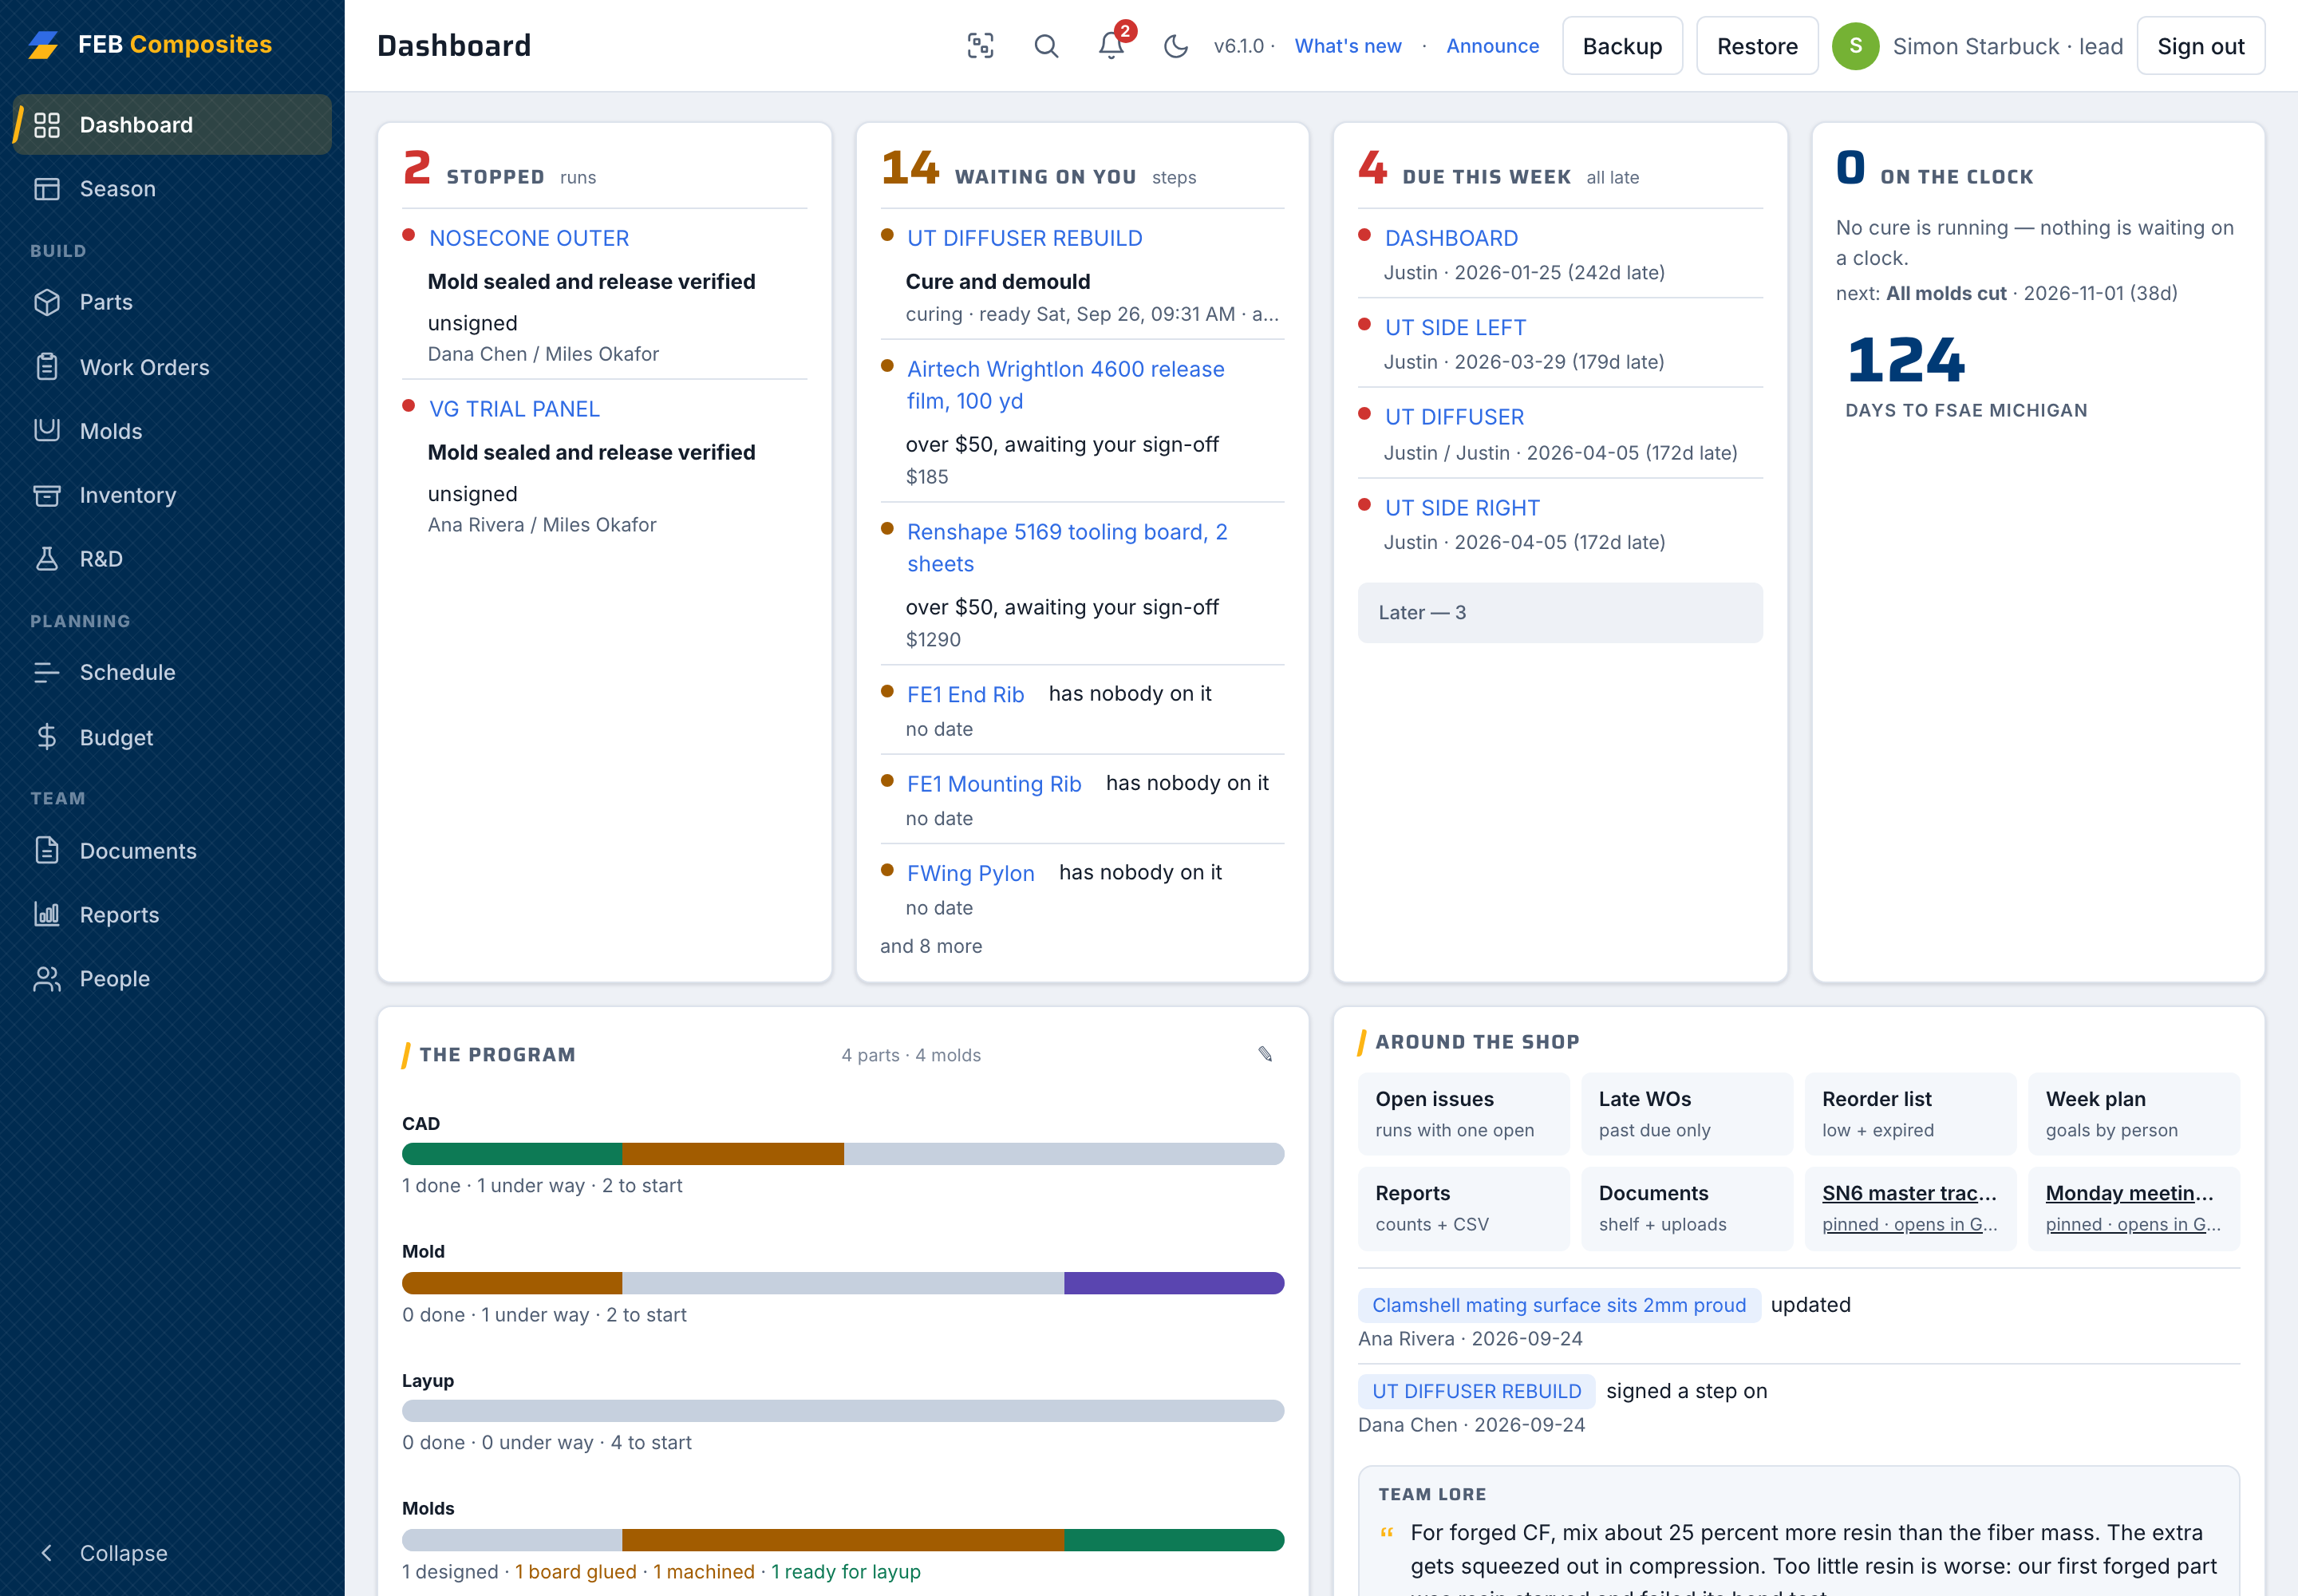
\includegraphics[width=\linewidth,trim=0 760 0 0,clip]{dashboard}\end{shot}

\vspace{6pt}
\renewcommand{\arraystretch}{1.5}
\begin{tabular}{@{}>{\headfont\color{red!70!black}}l@{\hspace{10pt}}p{0.8\linewidth}@{}}
Stopped          & A run that's stuck. Someone needs to unblock it before work continues.\\
\textcolor{orange!70!black}{Waiting on you} & \textbf{Your to-do list.} Steps you can sign right now, and purchases waiting on your OK.\\
\textcolor{red!70!black}{Due this week} & Deadlines in the next seven days, late ones first.\\
\textcolor{navy}{On the clock} & Cures running now, the next milestone, and days until competition.\\
\end{tabular}

\begin{tip}[Rule of thumb]
If “Waiting on you” is empty, check the week's plan on \g{timeline}\,\textbf{Schedule}
or ask in \#composites what needs a hand.
\end{tip}

\newpage
%% ---------------------------------------------------------------- 4 buy-off
\step{4}{Sign off a step (a “buy-off”)}

A \textbf{work order} is the traveler for one layup: the steps, the ply stack,
the materials, the photos. When you finish a step at the table, you sign it
in the app. That's a buy-off, and it records your name and the time.

\begin{shot}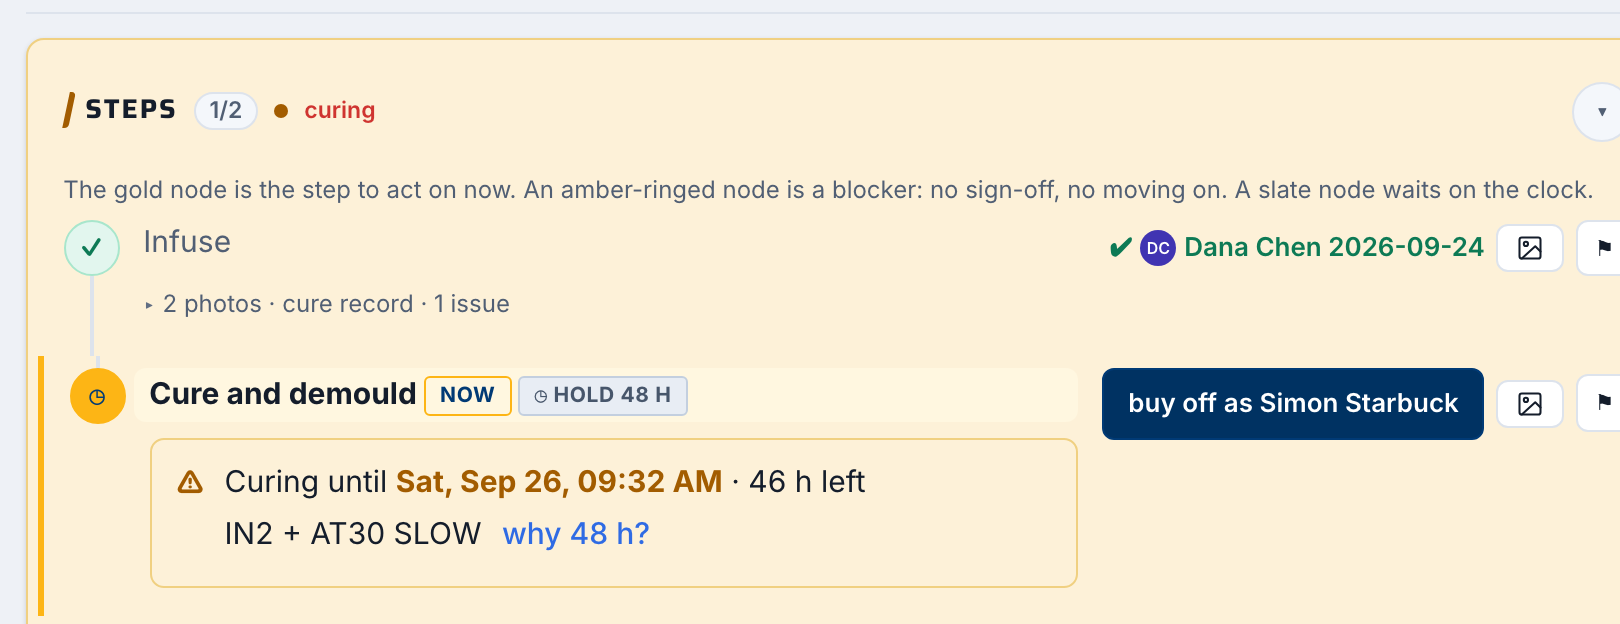
\includegraphics[width=\linewidth]{steps}\end{shot}

\vspace{4pt}
\begin{enumerate}[leftmargin=1.4em,itemsep=3pt]
  \item Open the work order (from the Dashboard, a search, or by scanning its label).
  \item The \textbf{gold dot} is the step to do now. Done steps show a
        \raisebox{-0.2em}{
\includegraphics[height=1em]{ic-check}} and who signed them.
  \item Do the step for real, then press \textbf{buy off as \emph{your name}}.
  \item If something is missing (a photo, a note, a linked CAD file) the app
        tells you what and gives you a button to add it. Nothing is lost by trying.
\end{enumerate}

\begin{minipage}[t]{0.48\linewidth}
\small\g{clock}\ \textbf{Cure hold.} A clock on a step means the resin is still
curing. The app won't let anyone sign until it's done. “why 48\,h?” explains
where the number came from.
\end{minipage}\hfill
\begin{minipage}[t]{0.48\linewidth}
\small\g{warning}\ \textbf{Something went wrong?} Press the flag next to a step
(or \textbf{Raise an issue}) and write what happened. That's what issues are
for, and nobody gets in trouble for one.
\end{minipage}

\vspace{18pt}
%% ---------------------------------------------------------------- cheat sheet
\begin{tcolorbox}[colback=paleblue,colframe=paleblue,arc=10pt,left=14pt,right=14pt,top=10pt,bottom=10pt,
  title={\headfont Cheat sheet},coltitle=white,colbacktitle=navy,fonttitle=\large]
\renewcommand{\arraystretch}{1.45}
\begin{tabular}{@{}p{0.47\linewidth}@{\hspace{16pt}}p{0.47\linewidth}@{}}
\key{Cmd}\,\key{K}\ \ search everything &
\g{plus}\ \textbf{New WO}\ \ start a work order \\
\g{edit}\ \textbf{Edit}\ \ change a record, then it saves as you go &
\g{print}\ \textbf{Print}\ \ a paper traveler for the table \\
\g{bell}\ \ someone @mentioned you &
\g{warning}\ \ raise an issue on a step \\
Click your avatar (top right) to set your photo &
\textbf{People} tab: change the name on your buy-offs \\
\end{tabular}
\end{tcolorbox}

\newpage
%% ---------------------------------------------------------------- 5 phone
\step{5}{At the shop, on your phone}

\begin{minipage}[t]{0.34\linewidth}
\vspace{0pt}
\begin{shot}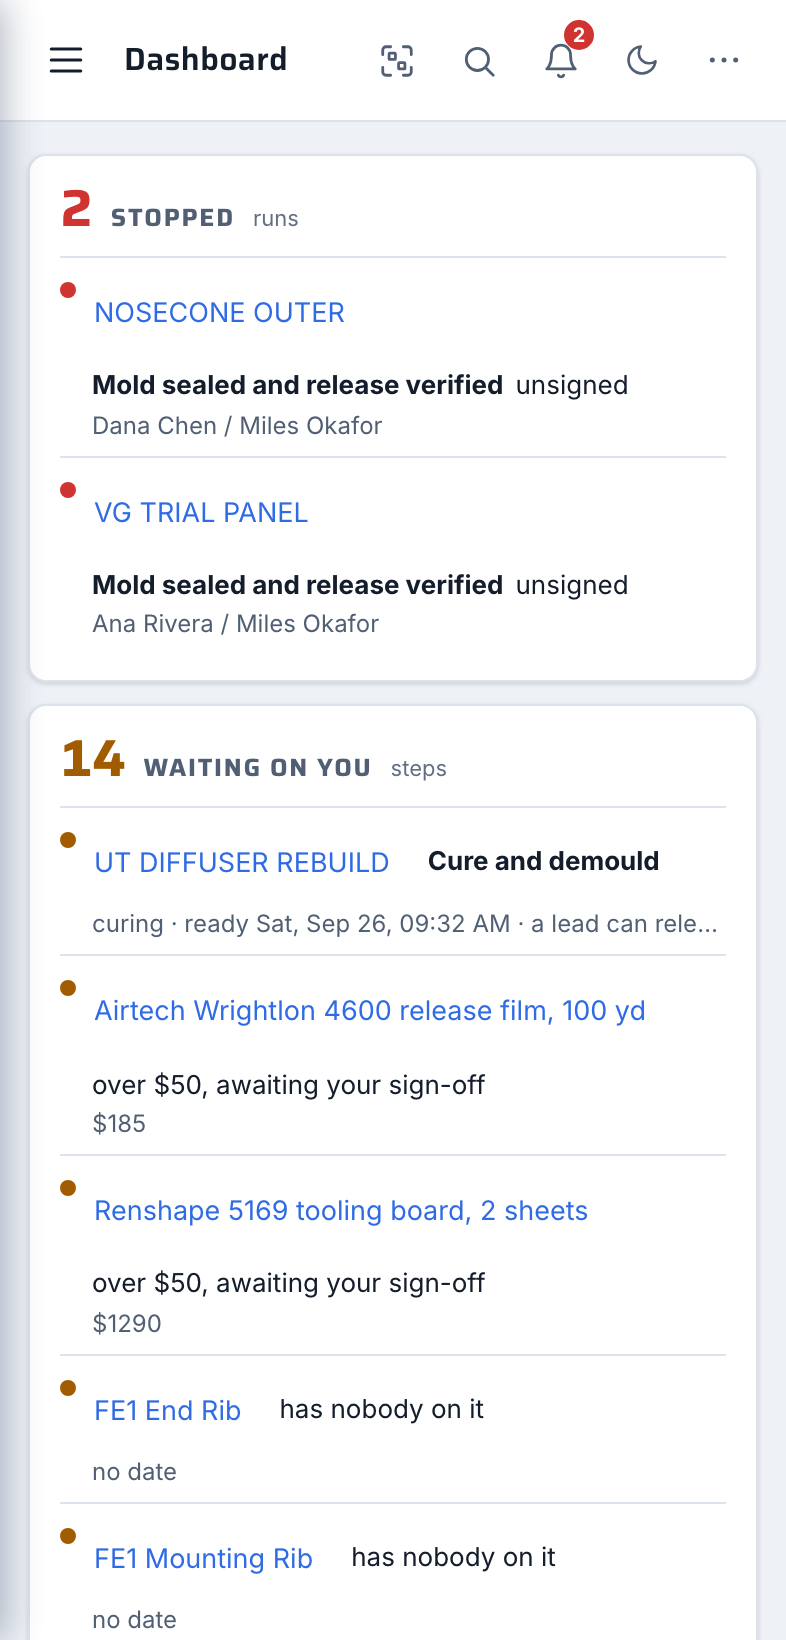
\includegraphics[width=\linewidth,trim=0 380 0 0,clip]{phone-dash}\end{shot}
\end{minipage}\hfill
\begin{minipage}[t]{0.61\linewidth}
\vspace{0pt}
The app works the same on a phone. The sidebar folds away behind
\g{menu}, and the account buttons move under \g{more}.

\vspace{4pt}
\textbf{Scanning labels.} Molds, boards and storage bins carry printed QR labels.
\begin{itemize}[leftmargin=1.2em,itemsep=3pt]
  \item \textbf{Signed in:} tap \g{scan} and point your camera at the label.
        The record opens.
  \item \textbf{Any phone camera:} scanning a label opens a public page with the
        part name, stage and location, even without an account or good signal.
\end{itemize}

\textbf{Photos.} Tap \g{image} next to a step to attach a picture of your
layup. It's never required, but it's the easiest way to show what you did.

\begin{tip}[Weak wifi at RFS]
The loading screen shows five lights. If one goes amber it tells you what's
stuck; \textbf{Continue anyway} still gets you in.
\end{tip}
\end{minipage}

\vspace{14pt}


\vspace{8pt}
\textbf{Stuck?} Ask in \textbf{\#composites} on Slack or grab a lead at the
Monday meeting. Nobody expects you to know the app on day one. The full manual
lives in the repo at \texttt{06 Composites App/app/README.md} if you ever
want the deep version.

\vfill
{\small\color{muted}Screenshots show sample data from app v6.1.0. Your screen
will have the team's real parts and names.}

\end{document}
